%!TEX root = ../../main.tex

\chapter{Fabrication of Nanodiamonds}	\label{ch::fabrication_nanodiamonds}
\chaptermark{Fabrication of Nanodiamonds}

	\enquote{Diamond forms under high temperature and pressure conditions that exist only about 100 miles beneath the earth's surface.} (Homepage of the Gemological Institute of America Inc.)
	While this statement is true for natural gem diamonds, various methods exist to synthetically produce diamond for applications in industry and research. 
	In this chapter, different fabrication methods of diamonds and \nds in particular are explained.
	The first two procedures described are the \hpht method and the \cvd are described.
	These are two of the most commonly used fabrication methods for laboratory-produced diamonds. 
	The \hpht (\HPHT) process mimics natural conditions under which diamond is formed within earth and is widely used to synthetically produce diamonds for industry.
	While these \HPHT diamonds are exploited for some experiments reported in this work, most measurements which are subject in this thesis are carried out on diamond produced with a \CVD process. 
	The third method which is described is the wet-milling process in a vibrational mill, which is a technique using \cvd or \HPHT diamond.
	\Nds produced with this milling process are the main focus of this thesis.
	It has to be stressed, that in contrast to the first two methods described in this chapter, the wet-milling process is not a process to produce diamond itself, rather it serves to crush bigger diamond starting material into pieces of a desired size.
	For a more extensive list of diamond production processes refer to e.g. \cite{davis1993diamond}.
	Aside from the general diamond fabrication processes, the production details of the \nds used for this thesis will be mentioned.
	% At the end, the methods of producing diamonds via detonation processes and sonicating graphite powders are briefly described.
	% As diamonds produced with this process is not scope of this thesis, they will only be shortly introduced to complete the list.

	

\section[HPHT]{High-Pressure High-Temperature Diamond}\label{sec::hpht}

	The \HPHT process was the first process to successfully synthesize diamond (in 1879).
	Temperatures of a few thousand degrees Celsius and pressures between \SI{50000}{bar} and \SI{100000}{bar} are needed \cite{davis1993diamond}.
	Today, it is still widely used due to its relatively cheap production costs \cite{wikiSyntheticDiamond}.
	\\
	In the \HPHT process, diamond is synthesized from graphite.
	The machine used for this kind of synthesis is a press.
	For some forms of this method, a metallic solvent is added which lowers the needed pressures; the solvent causes the graphite to dissolve at lower pressures and temperatures, and at the same time it causes the diamond to crystallize.
	Several press designs exist, which all provide a high temperature and a high pressure in their core.
	While it is possible to grow big (> \SI{10}{\carat}) high-quality diamonds with the \HPHT process, it is rather expensive when compared to the \CVD process due to the necessary high temperatures and high pressures.
	\\
	In the scope of this thesis, \HPHT diamonds \todo{sind die nicht auch zermahlen worden?}produced by Davydov et al. \cite{Davydov2014} are spectroscopically investigated.\todo[fancyline]{wie kommen da die SiVs rein?}


\section[CVD]{Chemical Vapor Deposition Diamond}\label{sec::cvd}

	\begin{figure}[tp]
		\begin{subfigure}[t]{ 0.49\linewidth}
			\caption{}\label{subfig::cvd_large}
			\centering
			\testbox{\includegraphics[trim = 0 0 0 0,  clip= true, height=5cm]{./pics/M05-13_191_131209_06.png}}
			% \caption{SEM picture of the milled nanodiamonds of a mean diameter of \SI{100}{\nano\meter}}
		\end{subfigure}
		\hfill
		\begin{subfigure}[t]{ 0.49\linewidth}
			\caption{}\label{subfig::cvd_detail}
			\centering
			\testbox{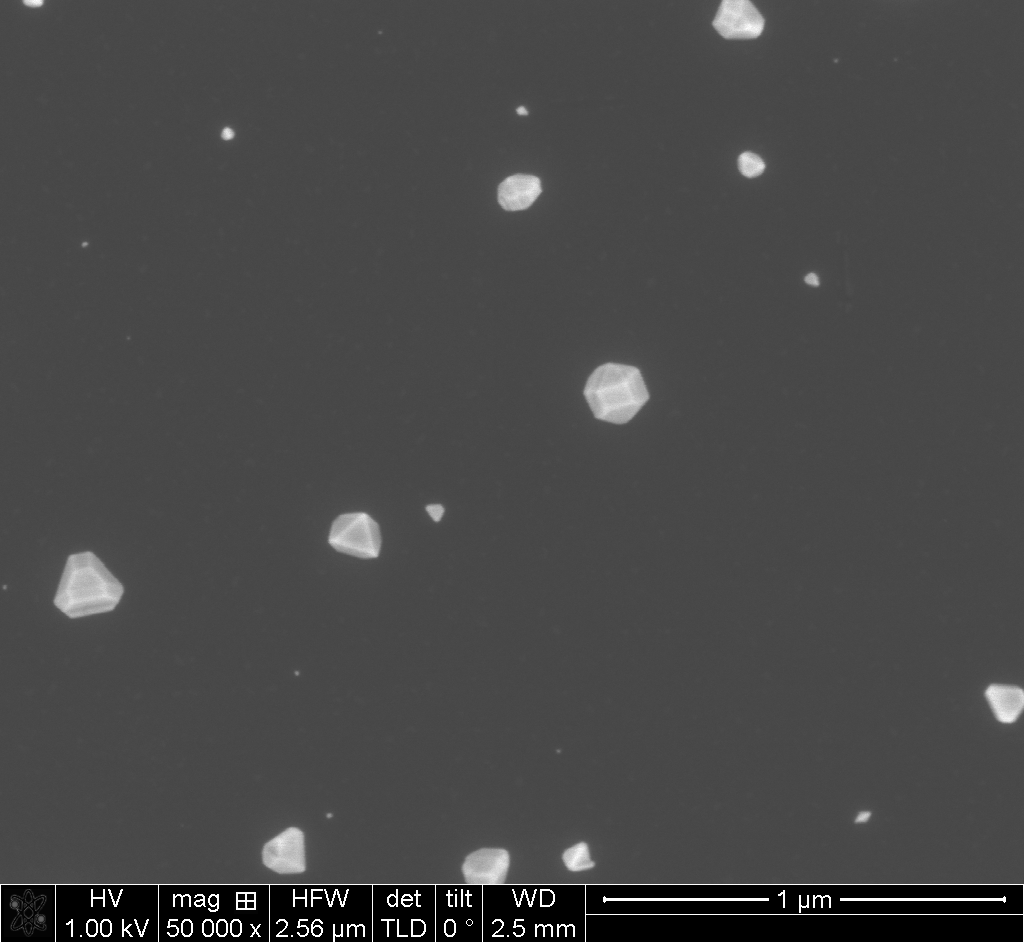
\includegraphics[trim = 0 0 0 0,  clip= true, height=5cm]{./pics/M05-13_191_131209_05.png}}
			% \caption{TEM picture of a \SI{100}{\nano\meter} diamond crystal.}
		\end{subfigure}
		\caption{SEM images of \CVD grown diamonds (sample \insitucvd) produced by M. Schreck's group (Augsburg University). The average size of these \nds is \SI{100}{nm}. (a) Overview image, white dots are \nds. (b) Detail image, it can be seen that not all \nds exhibit the same size and that they coexist in different shapes.}
		\label{fig::sem_cvd}
	\end{figure}

	\begin{figure}[tp]
		\centering
		\testbox{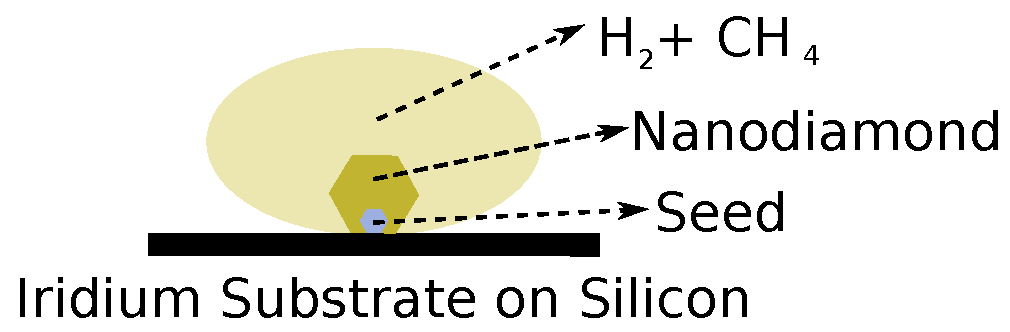
\includegraphics[trim = 0 0 0 0,  clip= true, width = 0.3\textwidth]{./pics/cvd_sketch.pdf}}
		\caption{Sketch showing the production of \CVD nanodiamonds in the growth chamber with a methane gas environment.}
		\label{fig::cvd_sketch}
	\end{figure}

	In contrast to the \HPHT process,  during the \cvd process, diamond is grown from a vapor phase.
	This process requires moderate temperatures (\SIrange{700}{1300}{\celsius}) but low pressures of less than \SI{1}{\bar} in a vacuum chamber \cite{}
	The diamond in a metastable state 
	Atomic hydrogen is necessary to suppress the simultaneous growth of graphite.
	The vapor phase within the growth chamber is a mixture of hydrogen and methane, the latter of which acts as a carbon source.
	Within the vacuum chamber, activation of the gas by an energy source (e.g. microwave plasma) breaks apart the gas molecules to release carbon atoms. 
	These atoms are drawn down toward the cooler substrate.
	On the substrate surface, various processes occur, such as adsorption, desorption and diffusion\todo{ueberleitung zu naechstem satz}.
	The growth parameters are optimized such that growth of diamond is favored \wrt graphite.
	\\
	Growth on a substrate is easier, if the lattice constant of the substrate and the crystal to be grown are very similar.
	The lattice constant of \ir (\SI{0.384}{nm}\cite{Arblaster2010,Gsell2007}) is very similar to the lattice constant of diamond (\SI{0.356}{nm}\cite{Davis1993}).
	Therefore, the diamonds were grown on a stratified substrate, consisting of \ir layers of \SIrange{60}{150}{nm} thickness grown onto an yttria-stabilized zirconia (YSZ) buffer layer, which in turn was grown on a silicon wafer \cite{Gsell2004a}.
	If the lattice constant of the substrate and the diamond are not matched, stress in the diamond lattice is induced.
	Therefore, the \ir substrate not only facilitates diamond growth, but also reduces unfavorable stress in the \nds (more on the effect of stress in \autoref{}).
	\\
	For crystals to form in heteroepitactic growth (i.e. one type of crystal is grown upon the surface of a different type), a nucleation step is necessary \cite{Schreck2014a}.
	The easiest method to obtain nuclei on a substrate is to spin-coat the substrate with small diamond seed crystals of a size of a few nanometers. 
	This method is exploited for all the \CVD grown \nds investigated in this thesis.
	Such small seed diamond crystals are commercially available, and are usually diamond particles produced by a so-called detonation process.
	In a detonation process, the high pressure produced by shockwaves of a detonation is used to create very small diamond particles of a size down to a few nanometers.
	During the \CVD growth process, carbon from the methane gas is adsorped \todo[fancyline]{is this correct?} to the seed crystals.
	To produce \nds of a desired size, the growth process is stopped when the diamonds grown onto the seed crystals reaches the desired size. 
	If the growth process is continued, the individual crystals grow together to form diamond films. 
	Such diamond films are used as starting material for the wet-milling process descirbed in the next section (\autoref{sec::wet_milled_nds})
	\\
	% There are two major different ways to make a plasma from the gas in the chamber: microwaves or a hot filament.
	% While the hot filament is easy to be technically implemented, it has th{}e disadvantage that atoms which are etched from the filament during the growth process is likely to contaminate the diamond.
	% This circumstance can mess up a clean signal from \sivs.
	% Therefore, we preferred diamonds grown with in a microwave plasma.
	One of the advantages of the \CVD process is that \si is incorporated \textit{in-situ}.
	This is achieved by etching of \si substrate edges by the \verify{plasma}which automatically occurs in the grows chamber and \si atoms diffuse into the methane gas. 
	For a higher \si content in the diamond, sacrificial \si is put into the growth chamber.
	These atoms are then build into the diamond lattice while growth.
	\\
	After \nd growth, the \nds are either investigated directly on the growth substrate or they are shaken off in an ultrasonic bath to obtain a solution which is coated onto other substrates for further measurements\todo[fancyline]{irgendwo einfuegen, was ich diesbezgl. gemacht hab}.
	\\
	In this thesis, two types of samples were investegated which were directly produced as nanodiamonds.
	\footnote{The \CVD nanodiamonds were grown by the group of M. Schreck \cite{}.}
	The first batch (henceforth called \CVD samples) were grown on detonation diamond seeds of a size smaller than \SI{3}{nm}(produced by the company Microdiamant, product Liquid Diamond monocrystalline, MSY {0-0.03} micron GAF).
	For the growth process, 1\% of methane is added to the hydrogen environment in the growth chamber.
	The growth process is performed with a pressure of \SI{30}{hPa} for \SIrange{30}{60}{min}, yielding \nds of a diameter of about \SIrange{100}{200}{nm}.
	\todo[fancyline]{put in figure}
	\\
	The other samples directly produced by a \CVD process are nanodiamonds grown onto molecular analogs of diamond crystals.
	A subgroup of these molecular diamonds are called diamondoids and are carbon crystals based on the carbon cage molecule adamantane \ch{C10H16}.
	The molecular diamonds used for this work are adamantane in cyclohexane, mercapto adamantane in cyclohexane, and cyclohexane.
	Each of these seed crystals is used in different growth processes.
	During the growth process, either 3\% or 1\% methane was added to the hydrogen plasma and either \si or \si dioxide was exploited to form \textit{in-situ} incorporated \sivs (see \autoref{tab::diamondiods}).


	\begin{table}[tp] 
		\centering 
		\caption{Summary of the samples grown on diamondoid seed crystals.} \label{tab::diamondiods} 
			\begin{tabular}{llll} 
			\toprule
			Sample name & Seed crystals & Methane conc. & \Si source \\ 
			\midrule
			160211\_E & Mercapto adamentane in cyclohexane & 1\% & \ch{SiO2} \\
			160211\_F & Cyclohexane                        & 1\% & \ch{SiO2} \\
			160212\_C & Cyclohexane                        & 3\% & \si         \\
			160212\_D & Adamentane in cyclohexane          & 3\% & \ch{SiO2} \\
			160212\_E & Mercapto adamentane in cyclohexane & 3\% & \ch{SiOs} \\
			160212\_F & Cyclohexane                        & 3\% & \ch{SiO2}\\
			\bottomrule
			\end{tabular} 
	\end{table}


\section[Wet-Milling]{Wet-Milled Nanodiamonds}\label{sec::wet_milled_nds}

	\begin{figure}[tp]
		\begin{subfigure}[t]{ 0.49\linewidth}
			\caption{}\label{subfig::sem_milled}
			\centering
			\testbox{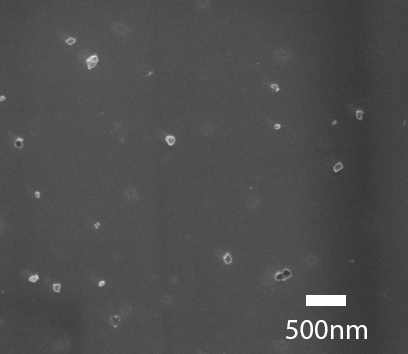
\includegraphics[trim = 0 0 0 0,  clip= true, height=5cm]{./pics/Ir27M_mitte_213_151111_22_crop.jpg}}
			% \caption{SEM picture of the milled nanodiamonds of a mean diameter of \SI{100}{\nano\meter}}
		\end{subfigure}
		\hfill
		\begin{subfigure}[t]{ 0.49\linewidth}
			\caption{}\label{subfig::tem_milled}
			\centering
			\testbox{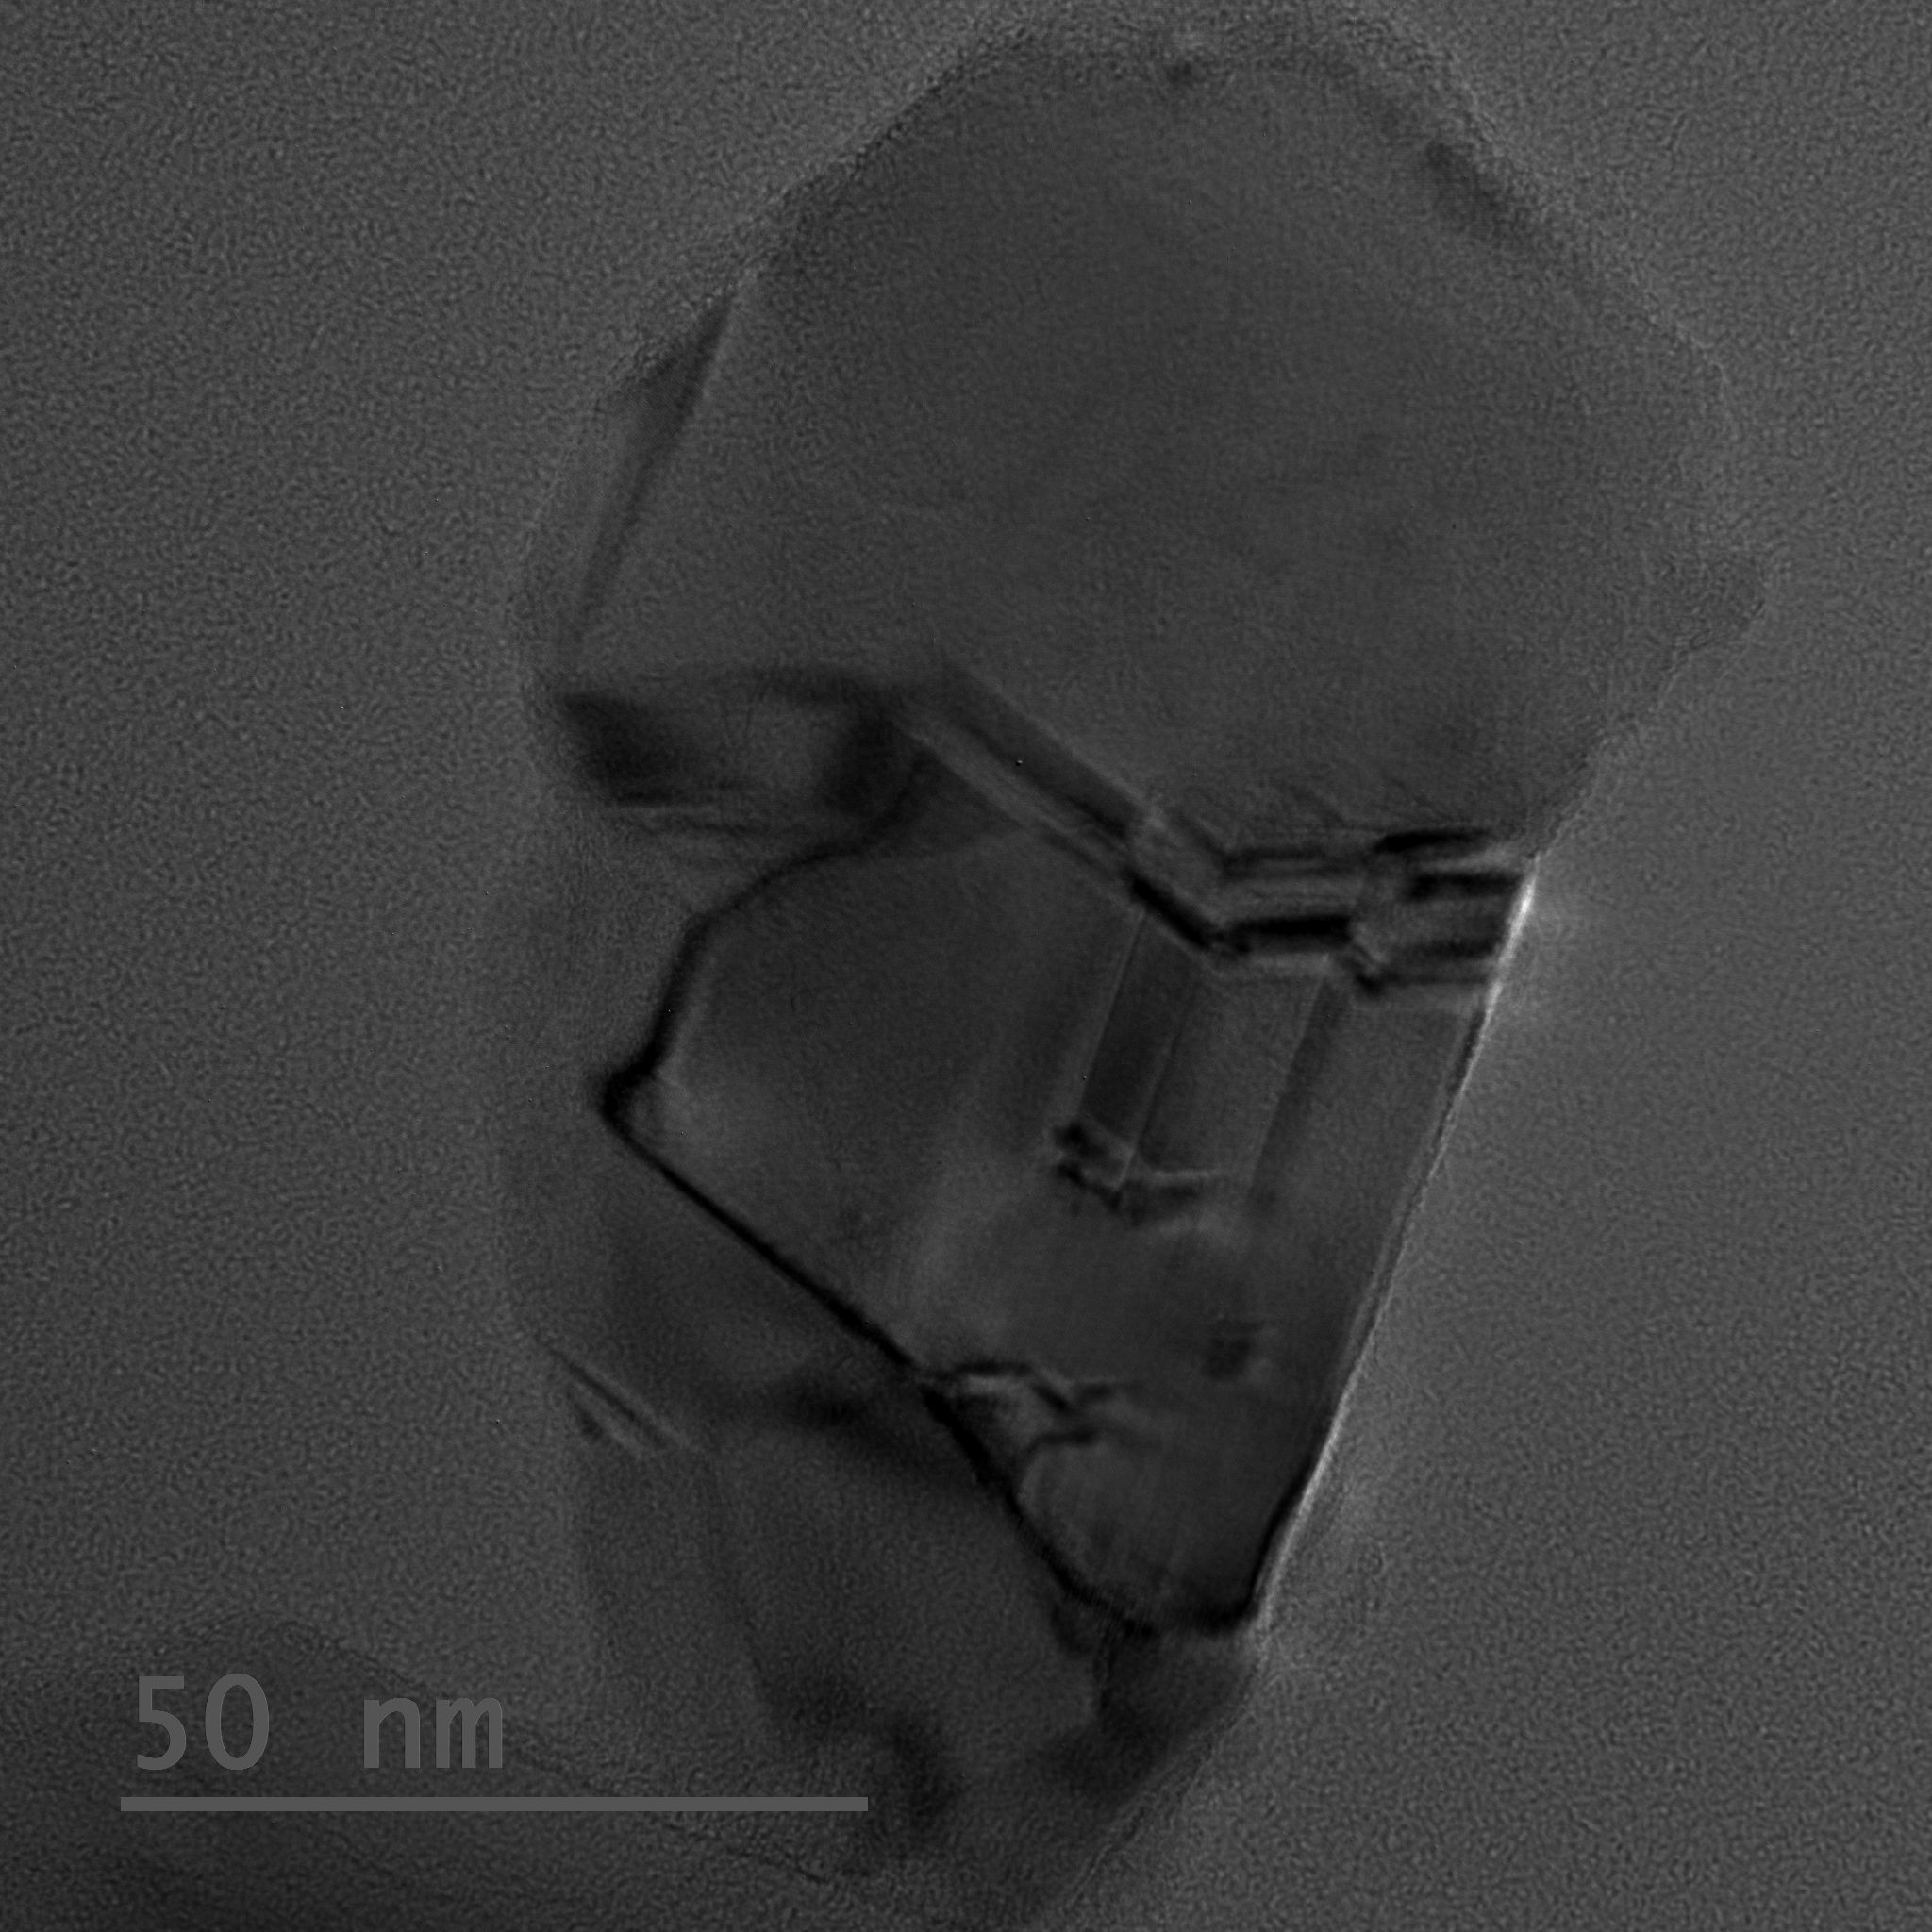
\includegraphics[trim = 0 0 0 0,  clip= true, height=5cm]{./pics/AM060-II-k4-2.png}}
			% \caption{TEM picture of a \SI{100}{\nano\meter} diamond crystal.}
		\end{subfigure}
		\caption{Pictures of the milled \nds (sample \insituH). (a) SEM picture showing the distribution of the \nd crystals on the \ir substrate. (b) TEM picture of a \nd particle.}
		\label{fig::semtem_millled}
	\end{figure}

	\begin{figure}[tp]
		\centering
		\testbox{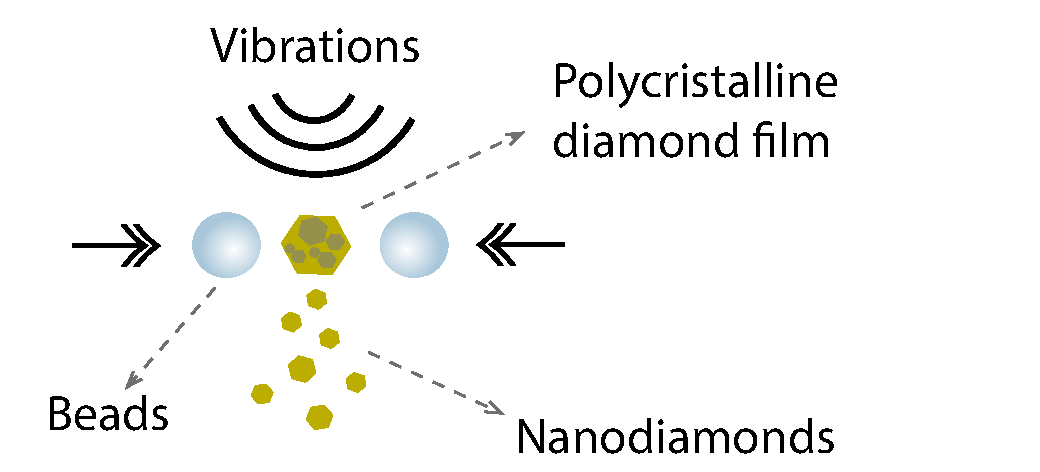
\includegraphics[trim = 0 0 0 0,  clip= true, width = 0.3\textwidth]{./pics/milling_sketch.pdf}}
		\caption{Sketch showing the wet-milling process in a vibrational mill. Vibrations from the mill drive the beads which collide with the diamond material and crush it to smaller pieces.}
		\label{fig::sketch_basd}
	\end{figure}

	Apart from growing \nds of a specific size directly via a \CVD process, macroscopic diamond starting material can be crushed to obtain small diamond particles.
	In contrast to \nds directly grown by a \CVD process, the process is divided into two sub-processes: 
	1. Diamond is produced, for example by an \HPHT process or by \CVD growth.
	2. The macroscopic diamond is milled to smaller diamond particles.
	For the wet-milling process which yields the \nds investigated in this thesis \footnote{If not otherwise stated, all the mentioned wet-milling wet-milling processes were carried out by Andreas Muzha in the group of A. Krueger (Julius-Maximilians Universit\"at W\"urzburg))}, small beads are used to crush the diamond material. 
	The beads are driven by vibrations of a vibrational mill\todo[fancyline]{info about vibrational mill}.
	A sketch of the process is shown in \autoref{fig::sketch_basd}\todo[fancyline]{more info}.
	\\
	The big advantage of the milling process is that it enables the production of a large quantity of diamond nanoparticles.
	When producing \nds directly via a \CVD process, the number of produced \nds in one process scales with the surface of the substrate on which the \nds are grown.
	In contrast, the quantity of milled \nds scales with the volume of the starting material
	Therefore in one and the same process the limit for the obtainable amount of diamond nanoparticles is much higher.
	Another advantage of the milling process is that the \nds are in an aqueous solution after milling.
	Therefore, it is viable to spin-coat the \nds directly onto any substrate suited for further experiments without further treatment.
	\\
	The wet-milled \nds have the disadvantage to contain grain boundaries, resulting in reduced crystal quality (\autoref{subfig::tem_milled}).
	While the polycristalline diamond film is more likely to break apart at grain boundaries, the final \nds still contain grain boundaries\todo{besser formulieren}.
	In contrast, as-grown \CVD \nds are mainly\todo{etwas anders fomulieren} single crystals. 
	\\
	After milling, the \nds are treated with post-processing steps including annealing in vacuum and oxidation in air.
	A detailed description of the processes and their impact is given in \ref{ch::crystal_quality}.
	\\
	In principle diamond produced by any production method can be used as starting material for the milling process.
	In the following sections, they are distinguished by the respective staring material and milling method.



	\subsection{Wet-Milled \HPHT \Nds}\label{subsec::milled_hpht_nds}
	We investigated \nds, which were produced from a \HPHT starting material and milled by a wet-milling process to median sizes of about \SIlist{45;80;260}{nm}.
	They were then drop-casted onto an \ir substrate and implanted with \ch{^{28}Si^1+} \todo[fancyline]{implantation parameters} \footnote{Implantation was performet by Dr. Detlef Rogalla at Ruhr-Universität Bochum (RUBION - Zentrale Einrichtung für Ionenstrahlen und Radionuklide)}.
	% After impalntation, the \nds of a size of \SI{80}{nm} (sample \hphtimpeighty) were annealed in vacuum for \SI{1}{\hour} at \SI{1000}{\celsius}, \SI{900}{\celsius} for \SI{3}{\hour}.
	At last, all \HPHT \nds (samples \hphtimpfortyfive, \hphtimpeighty,\hphtimptwosixty) were oxidized in air at SI{450}{\celsius} for \SI{3}{\hour}.
	\\

	\subsection{Wet-Milled \cvd \Nds}\label{subsec::milled_nds}
	% - milled CVD diamond film (in-situ SiV)
	In the following paragraphs, details of the production processes of \nd produced by wet-milling a \CVD diamond film in a vibrational mill are described. 
	For an overview of the samples refer to \autoref{tab::samplenames}.
	The starting material for the wet-milled \nds was a nanocristalline diamond film \cite{Williams2006a} directly grown on a silicon wafer by \CVD. 
	A microwave hydrogen plasma containing 1\% methane was used to grow on purified \SI{5}{\nano\meter} nanodiamond seeds (produced by PlasmaChem).
	To induce \textit{in-situ} \siv creation, sacrificial \Si pieces are situated in the growth chamber.
	During diamond growth the \si pieces are etched by the plasma and individual atoms are incorporated into the diamond lattice.
	The diamond film is then milled by a wet-milling process in a vibrational mill with steel beads.
	The high amount of steel containment due to the steel beads is removed by extensive acid treatment.
	We also investigated \nds milled with silicon nitride beads, and found that the choice of material of the beads does not cause any spectroscopic difference \autoref{}.
	The median diameters of the diamonds are \SIlist{50; 70; 100}{\nano\meter} (\autoref{subfig::sem_milled}).
	The particle sizes are determined with laser diffraction spectroscopy.
	Transmission Electron Microscopy (TEM) pictures of the diamond crystals show that the milled \nds are polycristalline, exhibiting a typical size of single crystals of a few tens of nanometers.
	In \autoref{subfig::tem_milled} a TEM image of a typical \nd is shown.
	Crystal boundaries have effects on the formation of color centers:
	\sivs are more prone to form at crystal boundaries \cite{Zapol2001}.
	The aqueous solution containing the \nds is drop cast onto an \ir film on a \Si substrate.
	The \ir film of a thickness of \SI{130}{nm} is grown onto a buffer layer of yttria-stabilized zirconia (YSZ) whith in turn is grown onto a \Si wafer.
	The \ir surface has the advantage that it acts as an antenna and therefore enhances the collection efficiency of fluorescence light \cite{Neu2012a} (for more information on the substrate see \autoref{sec::ir_substrate}).
	Post-procession treatment comprises either both annealing in vacuum at \SI{900}{\degreeCelsius} and consecutive \ox in air at a temperature of \SI{450}{\degreeCelsius}, or only one of the two methods.
	The duration for either treatment method was 3-6 hours.
	\\
	\subsection{Doubly Wet-Milled Implanted \Nds Implanted With \Si}\label{subsec::2_milled_nds}
	% - 2x vermahlene, implantierte NDs (E6->MDs->NDs)


	\begin{figure}[tp]
		\begin{subfigure}[t]{ 0.49\linewidth}
			\centering
			\testbox{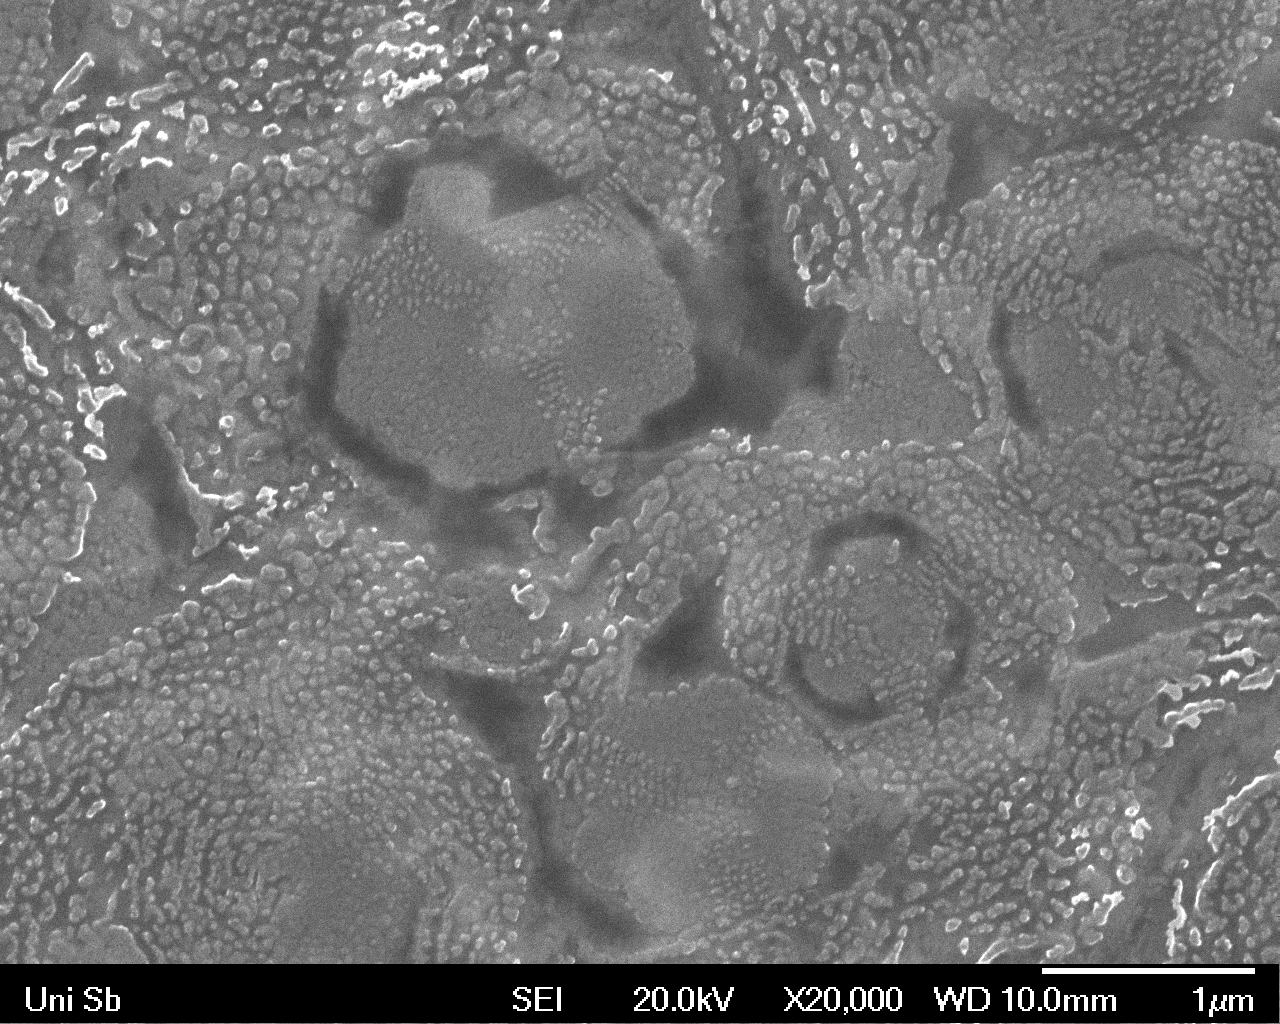
\includegraphics[trim = 0 0 0 0,  clip= true, width = \textwidth]{./pics/am21-sc-7-x20000-1.png}}
			\caption{}\label{subfig::sunken_nd}
		\end{subfigure}
		\hfill
		\begin{subfigure}[t]{ 0.49\linewidth}
			\centering
			\testbox{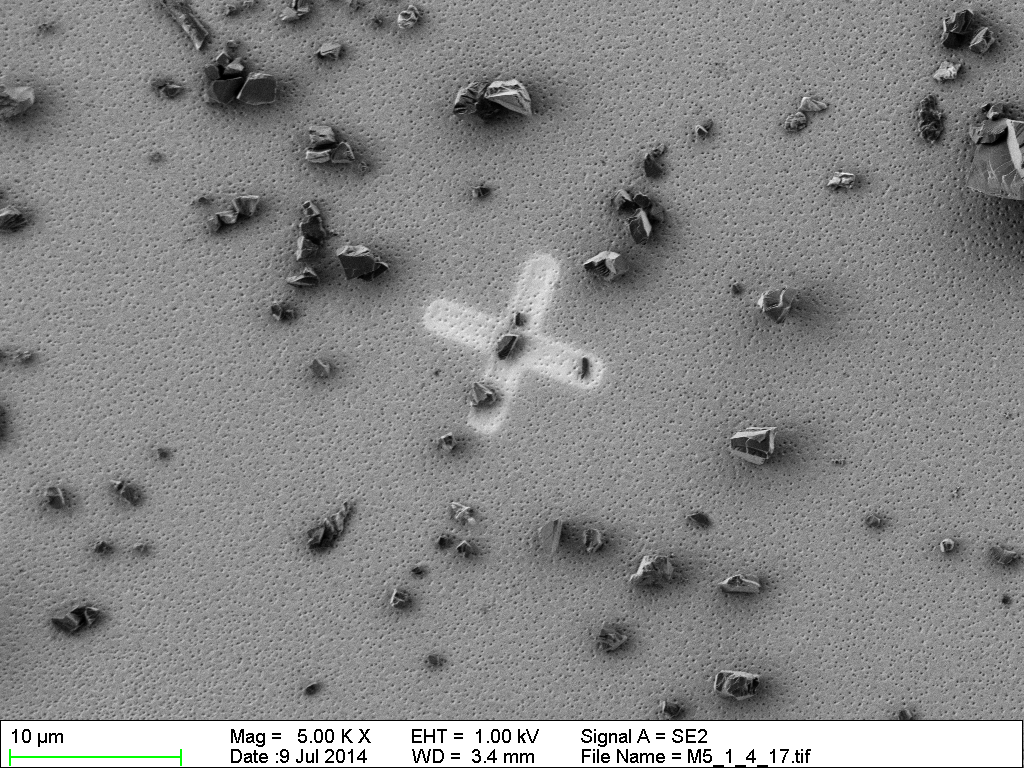
\includegraphics[trim = 0 0 0 0,  clip= true, width = \textwidth]{./pics/M5_1_4_17.png}}
			\caption{}\label{subfig::microdiamonds}
		\end{subfigure}
		\caption{(a) SEM picture of \nds sunken into a \si substrate after annealing at \SI{900}{\celsius} for \SI{3}{h}. Magnification \num{20000}. (b) SEM image of the microdiamonds after milling on an \ir substrate, but before implantation. In the middle of the picture, there is a reference cross milled into the \ir substrate with a focused ion beam. Its size amounts to \SI{10}{\micro\meter}. It can be seen, that the microdiamonds exhibit sizes of a few micrometer.}
		\label{fig::<fig>}
	\end{figure}

	We also investigated \nds with \sivs implanted after diamond growth. 
	Starting material was a polycristalline Element Six diamond film (electronic grade).
	In bulk material, the implantation causes the \sivs to form in a specific depth dependent on the implantation energy, leaving most of the diamond vacant of \sivs.
	As a consequence, a big portion of  \nds milled from such a bulk material would not host any \sivs.
	To obtain diamond particles with a homogeneous distribution of \sivs, the process of fabricating implanted \nds is the following. 
	First, the diamond film is milled to diamond particles of sizes of a few micrometers.
	In the second step, these microdiamonds are then spin-coated onto \ir substrates and implanted with \ch{^{28}Si^1+}.
	To eliminate lattice damage  and vacancies formed by the implantation process, the diamonds were annealed in vacuum and subsequently oxidized.
	At last, the micrometer sized diamond particles are milled to smaller sizes.

	\subsubsection{Preliminary Tests}\label{subsubsec::preliminary_tests}

	The starting material was an Element Six electronic grade diamond film.
	The diamond was milled in a wet-milling process to sizes on the order of micrometers, which were then coated onto a \si substrate.
	The microdiamonds were implanted with \ch{^{28}Si^1+} at an implantation energy of \SI{1.7}{MeV}, and fluences of \SIrange{e9}{e12}{cm^-1}\footnote{Implantation performed by Dr. Detlef Rogalla at RUBION - Zentrale Einrichtung f\"ur Ionenstrahlen und Radionuklide, Ruhr-Universit\"at Bochum mbH.}.
	After implantation, the microdiamonds on the \si substrate were annealed for \SI{2}{\hour} at \SI{900}{\celsius} and oxidized in air for another \SI{2}{\hour} at \SI{450}{\celsius}.
	However, we encountered the problem that the \si sublimated and re-nucleated during annealing, causing the diamonds to sink into the \si surface (\autoref{subfig::sunken_nd}).
	\Ir is less prone to damage by high temperatures and withstands annealing procedures up to our standard annealing temperature of \SI{900}{\celsius} without problems.
	Therefore, we used a sample with microdiamonds on a \si substrate which was not annealed to shake the \nds off the \si substrate in an ultrasonic bath, and consecutively coated the microdiamonds on an \ir substrate.
	After annealing and oxidizing the \nds on the \ir substrate, the \ir surface was intact.

	\subsubsection{Final Procedure}\label{subsubsec::final_procedure}

	For the milling process in a vibrational mill, a minimum amount of diamond material is necessary\todo{how much?}.
	When starting with a diamond film, this threshold is easily reached, however, a big quantity of microdiamonds is needed to meet the requirements.
	Therefore, production was carried out at a larger scale after the preliminary tests.
	The microdiamonds were directly spin-coated onto \ir substrates, implanted with \ch{^{28}Si^1+} (implantation energy \SI{900}{keV}, fluence \SI{e11}{\per\centi\meter\squared}) \footnote{Implantation performed by Jan Klug at rubitec - Gesellschaft f\"ur Innovation und Technologie der Ruhr-Universit\"at Bochum mbH.}
	The microdiamonds were then annealed in vacuum for \SI{3}{\hour} at \SI{900}{\celsius} and oxidized in air for \SI{3}{\hour} at \SI{450}{\celsius}.
	At last, they were milled again to sizes of about \SIlist{40;45;240;260}{nm}.
	The diamonds of sizes \SIlist{40;240}{nm} were annealed in vacuum at \SI{1200}{\celsius}\todo{time?}.

	



	\begin{table}[tp] 
		\centering 
		\caption{Summary of the wet-milled samples. The first column indicates the names of the samples, the second the mean diameter of the \nds, and the third describes how the \si was incorporated into the diamond.} \label{tab::samplenames} 
			\begin{tabular}{llll} 
			\toprule
			Sample name & Size & Si incorporation & Post-processing \\ 
			\midrule
			\hphtimpfortyfive & \SI{45}{nm} & \textit{implanted} & oxidized in air at \SI{450}{\celsius}\\ \hline 
			\hphtimpeighty & \SI{80}{nm} & \textit{in-situ} & \begin{tabular}[c]{@{}l@{}}annealed in vacuum for \SI{1}{\hour} at \SI{1000}{\celsius}\\ and at \SI{900}{\celsius} for \SI{3}{\hour}\end{tabular}\\ \hline 
			\hphtimptwosixty & \SI{260}{nm} & \textit{in-situ} & oxidized in air at \SI{450}{\celsius}\\ \hline 
			\insituF & \SI{50}{nm} & \textit{in-situ} & \begin{tabular}[c]{@{}l@{}}series of individual samples \\ with diverse post-processing steps\end{tabular}\\ \hline 
			\insituS & \SI{70}{nm} & \textit{in-situ} & \begin{tabular}[c]{@{}l@{}}series of individual samples \\ with diverse post-processing steps\end{tabular}\\ \hline 
			\insituSn & \SI{70}{nm} & \textit{in-situ} &  \begin{tabular}[c]{@{}l@{}}no post-processing \\ subset of \insituS \end{tabular}\\ \hline 
			\insituSo & \SI{70}{nm} & \textit{in-situ} & \begin{tabular}[c]{@{}l@{}}oxidized in air at \SI{450}{\celsius} \\ subset of \insituS \end{tabular}\\ \hline 
			\insituH & \SI{100}{nm} & \textit{in-situ} & \begin{tabular}[c]{@{}l@{}}series of individual samples \\ with diverse post-processing steps\end{tabular}\\ \hline 
			\insituHao & \SI{100}{nm} & \textit{in-situ} & \begin{tabular}[c]{@{}l@{}}annealed in vacuum at \SI{900}{\celsius}, \\ consecutively oxidized in air at \SI{450}{\celsius} \\ subset of \insituH \end{tabular}\\ \hline 
			\implantedTao & \SI{250}{nm} & implanted & \begin{tabular}[c]{@{}l@{}}annealed in vacuum at \SI{900}{\celsius}, \\ consecutively oxidized in air at \SI{450}{\celsius}\end{tabular}\\ \hline 
			\milltwofortyann & \SI{40}{nm} & implanted & \begin{tabular}[c]{@{}l@{}}annealed in vacuum at \SI{1200}{\celsius}, \\  consecutively oxidized in air at \SI{450}{\celsius}\end{tabular}\\ \hline 
			\milltwofiftyno & \SI{50}{nm} & implanted & oxidized in air at \SI{450}{\celsius}\\ \hline 
			\milltwotwofortyann & \SI{240}{nm} & implanted & \begin{tabular}[c]{@{}l@{}}annealed in vacuum at \SI{1200}{\celsius}, \\ consecutively oxidized in air at \SI{450}{\celsius}\end{tabular}\\ \hline 
			\milltwotwosixtyno & \SI{260}{nm} & implanted & oxidized in air at \SI{450}{\celsius}\\ 
			\bottomrule
			\end{tabular} 
	\end{table}




\section{\Ir Substrate}\label{sec::ir_substrate}


\begin{figure}[tp]
	\begin{subfigure}[t]{ 0.49\linewidth}
		\caption{}\label{subfig::wetting}
		\centering
		\testbox{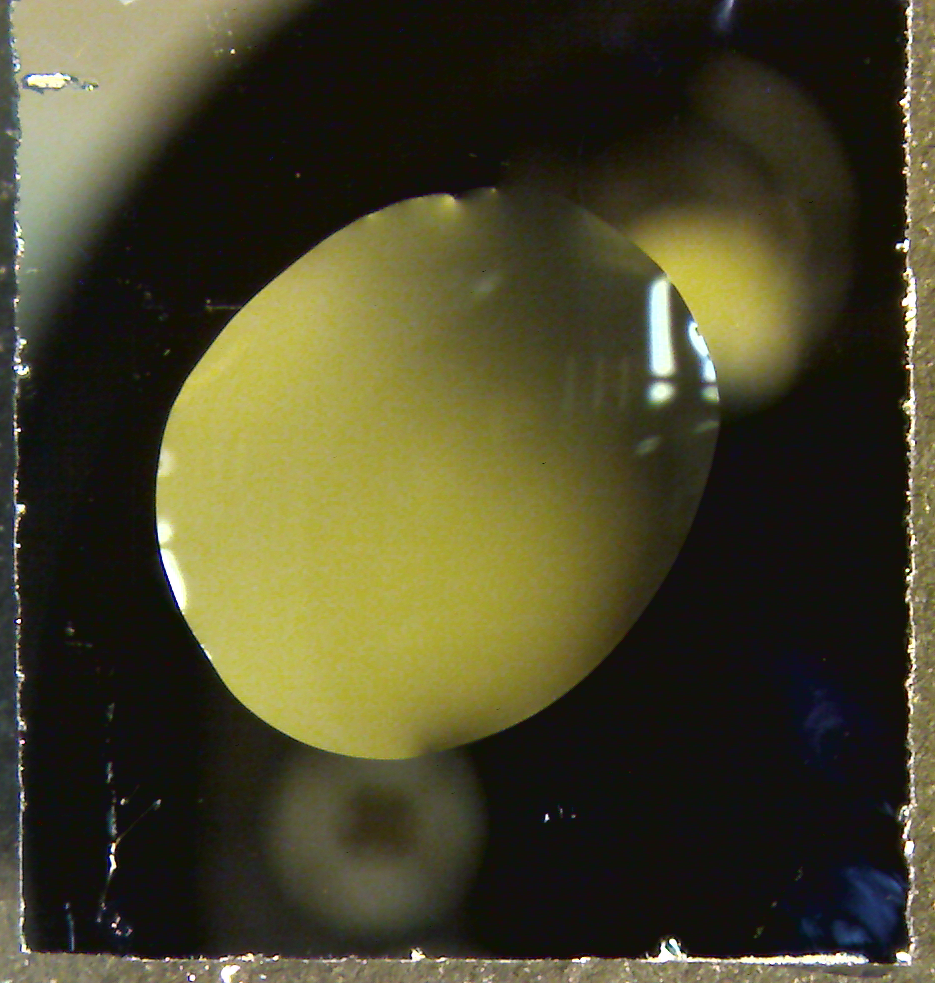
\includegraphics[trim = 0 0 0 0,  clip= true, width = \textwidth]{./pics/benetzung_M11_13_2edit.png}}
	\end{subfigure}
	\hfill
	\begin{subfigure}[t]{ 0.49\linewidth}
		\caption{}\label{subfig::peeled_ir}
		\centering
		\testbox{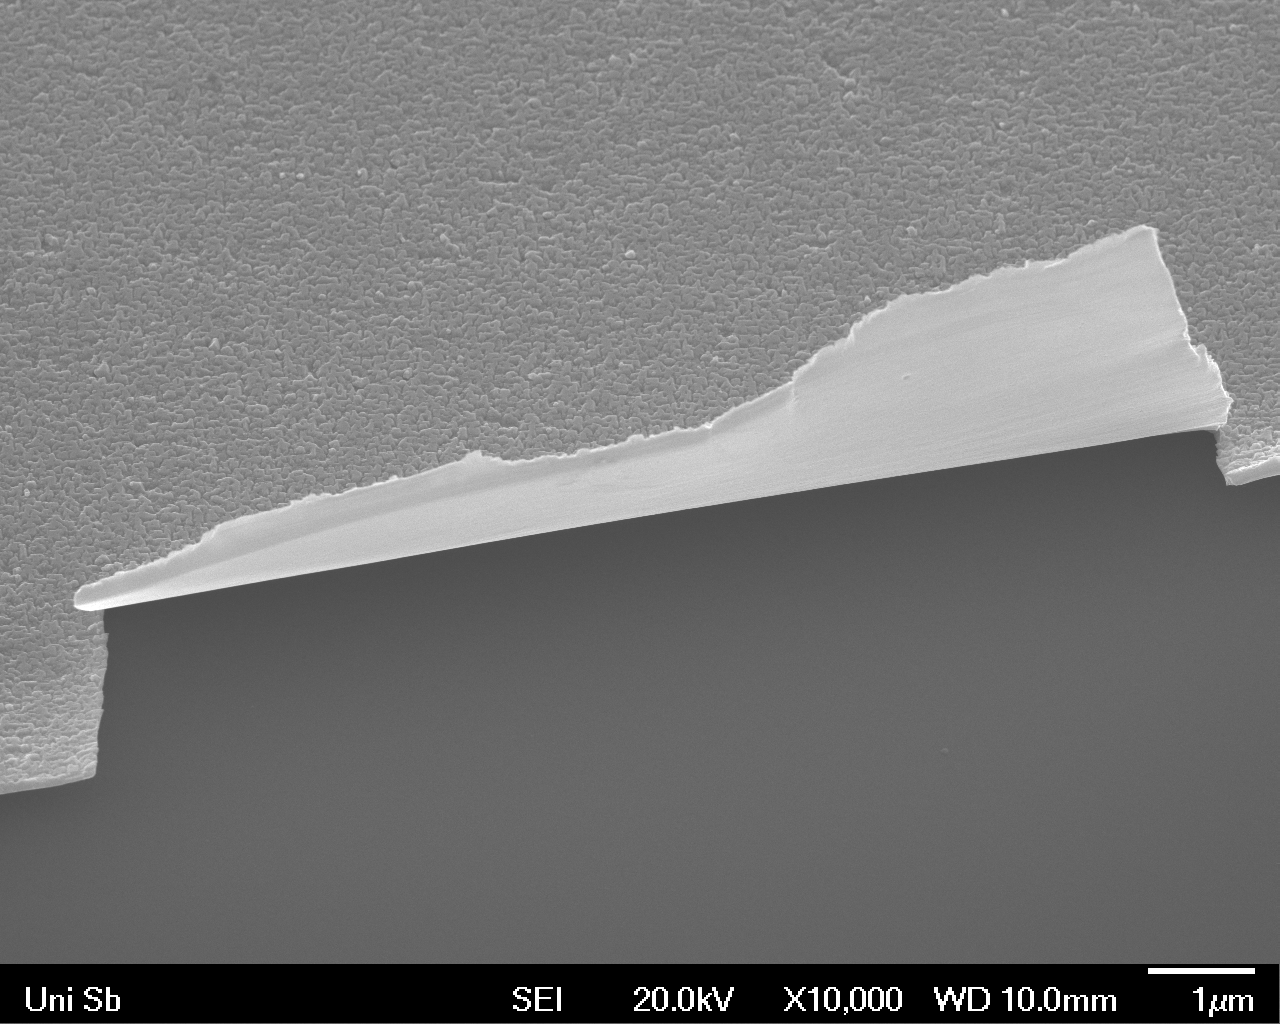
\includegraphics[trim = 0 0 0 0,  clip= true, width = \textwidth]{./pics/siq-basd-siv2-tilt45-x10000-1.png}}
	\end{subfigure}
	\caption{(a) Microcope image of a drop of water on an \ir substrate cleaned with Piranha etch. This picture was used to estimate the contact angle. (b) SEM picture of an \SI{60}{nm} \ir layer that peeled off the substrate after an ultrasonic bath.}
	\label{fig::sem_substrates}
\end{figure}

	As mentioned in \autoref{sec::cvd}, we used a \si substrate with an \ir layer on top for most experiments in order to match the lattice constant of diamond.
	We also use the same substrates for the experiments with wet-milled diamonds, as the \ir exhibits further advantages:
	\begin{itemize}
		\item The high hydrophilicity of \ir \todo[fancyline]{check numbers} enhances the homogenuity of the nanodiamonds on the substrate after spin-coating or drop-casting. 
		The hydrophilicity is further improved by treating the substrate in a Piranha etch (50:50 mixture of sulfuric acid \ch{H2So4} and hydrogen peroxide \ch{H2O2}) by removing oxide layers on the surface. 
		The treatment with Piranha etch also has the advantage that all organic contamination is removed.
		Measurements after applying the Piranha cleaning yielded an estimation of the contact angle of slightly more than one degree.
		To determine the contact angle with water, the volume of a water drop is compared to the surface it covers after dropping it onto an \ir substrate.
		From that an estimation of the contact angle is deduced.
		\item During the post-processing steps, it is of major importance, that the substrate can withstand high temperatures.
		As described in \autoref{subsubsec::preliminary_tests} during the preliminary tests with implanted nanodiamonds on a \si substrate (sample name \todo{sample name}), we encountered difficulties with diamonds on a \si substrate as the sunk into the surface after annealing.
		In contrast, \ir withstands the used annealing process without damage.
		\item Additionally to the mentioned technical advantages, another advantage of the \ir surface manifests itself during spectroscopic measurements: 
{}		\Ir acts both as a mirror and as an antenna for the \fl light emitted by the \siv \cite{Neu2012a}.
		Therefore, the collection efficiency of the \fl light is enhanced.
	\end{itemize}
	These advantages of \ir surfaces are only countered by one minor disadvantage:
	If the \ir layer is too thin, it tends to peel off the substrate (\autoref{subfig::peeled_ir}).
	We encountered this problem during a cleaning procedure in the ultrasonic bath.
	However, this disadvantage is easily circumvented by using a thicker \ir layer.
	For our measurements, we used an \ir layer of a thickness of \SI{130}{nm}, with which we did not encounter any adhesion problems.

	\subsection{Preparation of The Substrate}

	Prior to drop casting, the substrate is cleaned.
	The standard cleaning procedure comprised the following cleaning steps in an ultrasonic bath (\SIrange{3}{7}{\minute} each):
	\begin{itemize}
		\item Distilled water with a drop of dishwasher detergent
		\item Isopropanol (99.9\% p.a.)
		\item Acetone (99.9\% p.a.)
		\item Distilled water
	\end{itemize}
	Thereafter, the substrates are put into a Piranha solution (50\% sulfuric acid \ch{H2So4}, 50\% hydrogen peroxide \ch{H2O2}) to enhance the surface hydrophilicity and therefore obtain a homogeneous distribution of diamonds on the surface.
	They are then put again into distilled water and blown dry with compressed air to avoid residue from the water.
	The substrates were then either drop-casted or spin-coated with aqueous diamond solutions.
	For the prior, the substrates are heated to a temperature of \SI{60}{\celsius} and drops of a volume of about \SI{5}{\micro\liter} dropped onto the substrate.
	If substantially more than \SI{5}{\micro\liter} is needed, the several drops of about \SI{5}{\micro\liter} are dropped onto the substrate consecutively, as with a single big drop the solution would flow off the substrate before drying.
	For spin-coating, a home built spin coater was used.
	Drops of \SI{5}{\micro\liter} are dropped on the substrate and the spin-coater set to a velocity of \SI{2500}{\rpm} for \SI{3}{\minute}.